% !TeX encoding = UTF-8 Unicode
% !TEX root = MaksimenkoThesis.tex

\chapter{Основные понятия}

В этой главе приводятся определения и перечисляются известные факты, служащие основой для изложения результатов диссертации в последующих главах.
В~разделах~\ref{sec:graphs} и~\ref{sec:polytopes} вводятся необходимые понятия 
теории графов и теории выпуклых многогранников, соответственно.
В~разделе~\ref{sec:complexity} уточняются некоторые понятия теории сложности вычислений %задач и алгоритмов 
и, в частности, теории NP-полных задач. Общепринятая формулировка задачи комбинаторной оптимизации уточняется в разделе~\ref{sec:CO}.
%Понятие многогранника (полиэдра) задачи вводится в разделе~\ref{sec:ProblemPolytopes}, там же приводятся многочисленные примеры. Раздел~\ref{sec:Survey} посвящен обзору известных результатов по данной теме.
%В частности, в нем широко представлены результаты о свойствах графов многогранников задач, а также о расширенных формулировках многогранников.
%В~разделе~\ref{sec:questions} формулируются общие вопросы, ответы на которые будут представлены в последующих главах.


\section{Множества и графы}
\label{sec:graphs}

\subsection{Множества}

%Множество натуральных чисел обозначаем через $\N$.
Для множества $\{1,2,\dots,n\}$, где $n\in \N$, будем пользоваться обозначением~$[n]$. 
Целую часть %Наибольшее целое, не превосходящее 
действительного числа $x$ обозначаем $\lfloor x \rfloor$.
Наименьшее целое, большее или равное числа $x$, обозначаем $\lceil x\rceil$.

Пусть $E$ "--- некоторое конечное множество. 
Множество всех подмножеств множества $E$ обозначается $2^E$.
\emph{Характеристическим вектором} подмножества $T \in 2^E$ называется 0/1"~вектор $v = \chi(T) \in \{0,1\}^E$ с координатами
\[
v_{e} = \begin{cases}
1,& \text{если $e\in T$,}\\
0,& \text{если $e\in E\setminus T$.}
\end{cases}
\]
Если же элементы множества $E$ пронумерованы, то характеристический вектор может быть определен как $v = \chi(T) \in \{0,1\}^{|E|}$ с координатами
\[
v_{i} = \begin{cases}
1,& \text{если $e_i\in T$,}\\
0,& \text{если $e_i\in E\setminus T$.}
\end{cases}
\]
%Таким образом, вершины любого 0/1-многогранника в $\R^d$ можно интерпретировать как характеристические векторы некоторых подмножеств $d$-элементного множества $S$.


\subsection{Графы}
\emph{Графом} или \emph{неориентированным графом} называется упорядоченная пара $G = (V, E)$,
где $V$ "--- конечное множество, а $E$ "--- некоторое множество двухэлементных подмножеств множества $V$.
Элементы множества $V$ называются \emph{вершинами} графа $G$, а элементы множества $E$ "--- его \emph{ребрами}.
Вершины $v$ и $u$ называются \emph{концами} ребра $\{v,u\}$.
Все рассматриваемые в диссертации графы не содержат кратных ребер (множество $E$ не содержит одинаковых элементов) и петель (концы любого ребра $e \in E$ являются разными вершинами).
Граф называется \emph{полным,} если каждая пара его вершин образует ребро этого графа.
%Полный граф на $n$ вершинах обозначается $K_n$.

Вершины $v$ и $u$ графа $G = (V,E)$ называются \emph{смежными} в $G$, если $\{v,u\} \in E$.
Если же $\{v,u\} \notin E$, то вершины $v$ и $u$ называются \emph{несмежными.}
\emph{Степенью} вершины $v \in G$ называется число смежных с ней вершин.
Граф, степень каждой вершины которого равна трем, называется \emph{кубическим.}
Подмножество вершин $V' \subseteq V$ называется \emph{кликой} в графе $G$, если любые две вершины из $V'$ смежны.
Максимальный размер (мощность) клики в $G$ называется \emph{кликовым числом} графа $G$ и обозначается $\omega(G)$.
Подмножество вершин $V' \subseteq V$ называется \emph{независимым} в графе $G$, если любые две вершины из $V'$ несмежны.

Пусть $G' = (V', E')$ "--- еще один граф.
Графы $G$ и $G'$ называются изоморфными, если существует взаимно"=однозначное отображение $f \from V \to V'$ такое,
что $\{v, u\} \in E$ тогда и только тогда, когда $\{f(v), f(u)\} \in E'$.
Граф $G'$ называется \emph{подграфом} графа $G$, если $V' \subseteq V$ и $E' \subseteq E$.
Далее, для краткости, любой граф $G'$ изоморфный подграфу графа $G$ будем называть подграфом графа $G$.
Подграф $G'$ графа $G$ называется \emph{порожденным} или \emph{индуцированным}, если $\forall v, u \in V'$ из $\{v, u\} \in E$ следует $\{v, u\} \in E'$.

\emph{Путем} в графе $G$ называется множество ребер вида 
\[P = \{\{v_1, v_2\}, \{v_2, v_3\}, \dots, \{v_{k-1}, v_k\}\},
\] 
где $v_1$, $v_2$, \dots, $v_k$ "--- попарно различные вершины, $k \ge 2$.
В таком случае будем говорить, что путь $P$ \emph{соединяет} вершины $v_1$ и $v_k$, и называть его \emph{$v_1$-$v_k$ путем}.
Граф называется \emph{св\'{я}зным}, если любые две его вершины соединяет некоторый путь в этом графе.
Путь в графе $G$ называется \emph{гамильтоновым}, если каждая вершина графа принадлежит хотя бы одному ребру этого пути.
%\emph{Длиной} пути называется число составляющих его ребер.
\emph{Расстоянием} между вершинами $v$ и $u$ в графе $G$ называется наименьшее число ребер в соединяющем их пути;
если же такой путь не существует, то расстояние полагается равным~$+\infty$.
\emph{Диаметром} $\diam(G)$ графа $G$ называется наибольшее расстояние между его вершинами (выбор осуществляется среди всех пар вершин).

\emph{Циклом} в графе $G$ называется множество ребер вида 
\[
C = \{\{v_1, v_2\}, \{v_2, v_3\}, \dots, \{v_{k-1}, v_k\}, \{v_k, v_1\}\},
\] 
где $v_1$, $v_2$, \dots, $v_k$ "--- попарно различные вершины, $k \ge 3$.
Цикл в графе называется \emph{гамильтоновым}, если каждая вершина графа принадлежит ровно двум ребрам этого цикла.
Если в графе есть гамильтонов цикл, то и сам граф называется \emph{гамильтоновым.}
Граф без циклов называется \emph{лесом}, а связный лес "--- \emph{деревом}.

Вершина $v$ и ребро $e$ называются \emph{инцидентными}, если $v\in e$.
\emph{Матрицей инциденций} вершин"=ребер графа $G = (V,E)$ называется матрица $M \in \{0,1\}^{n\times k}$, $n = |V|$, $k = |E|$, элементы которой определяются следующим образом:
\[
M_{ij} = 
\begin{cases}
1, &\text{если $v_i\in e_j$,}\\
0, &\text{иначе.}
\end{cases}
\]

Будем говорить, что подмножество ребер $E' \subseteq E$ \emph{покрывает} вершины $V$,
если каждая вершина $v \in V$ инцидентна хотя бы одному ребру из $E'$.
Аналогично, подмножество вершин $V' \subseteq V$ \emph{покрывает} ребра $E$,
если каждое ребро $e \in E$ инцидентно хотя бы одной вершине из $V'$.

Два ребра в графе называются \emph{смежными}, если они содержат общую вершину, в противном случае они называются \emph{несмежными.}
Множество попарно несмежных ребер графа называется \emph{паросочетанием}. 
Паросочетание, покрывающее все вершины графа, называется \emph{совершенным.} 
Таким образом, совершенное паросочетание может быть только у графов с четным числом вершин.

\emph{Разрезом} в графе $G = (V, E)$ называется множество ребер вида 
\[
\delta(U) \coloneqq \Set*{\{u,v\} \in E \given u\in U,\ v\in V \setminus U}, \quad \text{где } U \subseteq V. 
\]
Из определения следует, что $\delta(U) = \delta(V \setminus U)$.
Разрез $\delta(U)$ называется \emph{$s$-$t$ разрезом}, если $s \in U$ и $t \in V\setminus U$\label{def:stcut}.
%\emph{Разбиением множества} $X$ называется набор его попарно непересекающихся подмножеств, объединение которых совпадает с $X$.
Граф $G = (V, E)$ называется \emph{двудольным}, если множество его вершин $V$ можно разбить на две \emph{доли} $U$ и $V \setminus U$ так, что $\delta(U) = E$. 
Двудольный граф называется \emph{полным двудольным}, если $\{u, v\} \in E$ для любых $u \in U$ и $v \in V \setminus U$.


Граф $G = (V,E)$ называется \emph{реберно"=взвешенным}, если на множестве его ребер $E$ задана функция весов $f \from E \to \R$.
Число $f(e)$ называется \emph{весом} ребра $e \in E$.
\emph{Весом подмножества} $E' \subseteq E$ или \emph{подграфа} $G' = (V', E')$ реберно"=взвешенного графа $G$ называется сумма весов входящих в него ребер.
Граф $G$ называется \emph{вершинно"=взвешенным}, если задана функция $g \from V \to \R$.
В таком случае число $g(v)$ называется \emph{весом} вершины $v \in V$, а \emph{весом подмножества} $V' \subseteq V$ называется сумма весов входящих в него вершин.

\subsection{Орграфы}

\emph{Ориентированным графом} или \emph{орграфом} называется упорядоченная пара $D = (V, A)$, где $V$ "--- конечное множество, называемое \emph{множеством вершин}, $A$ "--- некоторое множество упорядоченных пар вершин, называемых \emph{дугами}. 
Также, как и для графов, далее предполагаем, что в $A$ нет кратных дуг и петель.
Большинство перечисленных выше понятий для графов переносится (иногда с небольшими уточнениями) на орграфы.

Пусть $(v, u) \in A$.
Вершина $v$ называется \emph{началом} дуги $(v, u)$, а вершина $u$ "--- ее \emph{концом}.
Каждая из этих вершин и дуга $(v, u)$ называются \emph{инцидентными} друг другу.
Орграф будем называть \emph{полным,} если каждая упорядоченная пара его вершин образует дугу этого графа, то есть $|A| = |V| (|V| - 1)$.
%Орграф называется \emph{турниром,} если для любой (неупорядоченной) пары вершин $u,v \in V$ ровно одна из дуг $(u, v)$ и $(v, u)$ принадлежит $A$.

\emph{Орпутем} или просто \emph{путем} в орграфе $D$ будем называть множество дуг вида 
\[P = \{(v_1, v_2), (v_2, v_3), \dots, (v_{k-1}, v_k)\},
\] 
где $v_1$, $v_2$, \dots, $v_k$ "--- попарно различные вершины, $k \ge 2$.
Вершины $v_1$ и $v_k$ называются, соответственно, \emph{началом} и \emph{концом} пути $P$, 
а вершины $v_2$, \dots, $v_k$ "--- его \emph{внутренними вершинами}.

\emph{Контуром} в орграфе $D$ называется множество дуг вида 
\[
C = \{(v_1, v_2), (v_2, v_3), \dots, (v_{k-1}, v_k), (v_k, v_1)\},
\] 
где $v_1$, $v_2$, \dots, $v_k$ "--- попарно различные вершины, $k \ge 2$.
Орграф, не содержащий контуров, называется \emph{ациклическим.}

\emph{Разрезом} в орграфе $D = (V, A)$ называется множество дуг вида 
\[
\delta^+(U) \coloneqq \Set*{(u,v) \in A \given u\in U,\ v\in V \setminus U}, \quad \text{где } U \subseteq V. 
\]
Разрез $\delta^+(U)$ называется \emph{$s$-$t$ разрезом}, если $s \in U$ и $t \in V\setminus U$\label{def:stdicut}.

\begin{comment}
Орграф $D = (V, A)$ называется \emph{транзитивным}, если из условий $(v, u) \in A$ и $(u, w) \in A$ следует $(v, w) \in A$.
Так как мы не рассматриваем графы с петлями, то из транзитивности следует ацикличность.
Таким образом, множество дуг транзитивного графа задает частичный порядок на множестве вершин графа и, наоборот, каждый частичный порядок может быть представлен множеством дуг некоторого транзитивного графа.
Если для каждой пары вершин $u,v \in V$ в множество $A$ входит ровно одна из двух дуг $(v, u)$ и $(u, v)$, то соответствующий орграф называется \emph{турниром}.\label{def:linearOrdering}
Транзитивный турнир задает линейный порядок на множестве вершин.
Поэтому далее, говоря о частичном (линейном) порядке мы часто будем подразумевать соответствующий транзитивный орграф (турнир).
\end{comment}

\section{Многогранники}
\label{sec:polytopes}

%В этом разделе перечисляются некоторые .
При изложении основополагающих понятий и фактов теории выпуклых многогранников будем придерживаться терминологии монографий~\cite{Emelichev:1981} и~\cite{ZieglerBook}.


Под $\R^d$ будем понимать пространство всех вектор"=столбцов длины $d$ с вещественными координатами. 
Сами вектор-столбцы из $\R^d$ будем выделять полужирным шрифтом: $\bm{x}, \bm{x_1}, \bm{y}, \bm{z} \in \R^d$.
Вектор"=столбцы, составленные из одних нулей или же одних единиц, будем обозначать $\bm{0}$ и $\bm{1}$ соответственно
(их размерность ясна из контекста везде, где они будут использоваться).
Единичные векторы, образующие канонический базис в $\R^d$, обозначаем $\bm{e_1}$, \dots, $\bm{e_d}$
(таким образом, $\sum_{i\in[d]} \bm{e_i} = \bm{1}$).
Следуя общепринятой практике~\cite{ZieglerBook},  вектор"=столбцы часто будут называться точками.


\emph{Гиперплоскостью} в~$\R^d$ называется множество
\[
H(\bm{a},b) \coloneqq \Set*{\bm{x}\in\R^d \given \bm{a}^T \bm{x} = b}, 
%\qquad \bm{a}\in\R^d, \ \bm{a} \ne \bm{0}, \ b\in\R,
\]
где $\bm{a} \in \R^d$ "--- вектор нормали гиперплоскости, $\bm{a} \ne \bm{0}$, а число $b \in \R$ определяет величину смещения гиперплоскости относительно начала координат,
$\bm{a}^T \bm{x}$ "--- матричное произведение вектор"=строки $\bm{a}^T$ на вектор"=столбец $\bm{x}$, или, другими словами, скалярное произведение $\langle\bm{a},\bm{x}\rangle$.


Линейная комбинация $\sum_{i\in[n]} \lambda_i \bm{x_i}$ точек $\bm{x_1}$, \dots, $\bm{x_n}$ из $\R^d$,
где $\lambda_i \in \R$, $i\in[n]$,
называется \emph{аффинной комбинацией},
если $\sum_{i\in[n]} \lambda_i = 1$.
\emph{Аффинной оболочкой} $\aff(X)$ непустого множества $X \subseteq \R^d$ называется множество всех аффинных комбинаций каждого набора точек из $X$.
Множество точек называется \emph{аффинно независимым}, если ни одна точка этого множества не принадлежит аффинной оболочке остальных его точек.
\emph{Аффинной размерностью} множества $X$ называется мощность аффинно независимого подмножества $S \subseteq X$ минус один, при условии $\aff(S) = \aff(X)$. В частности, аффинная размерность пустого множества равна $-1$.
\emph{Размерность} $\dim(X)$ множества $X$ полагаем равной его аффинной размерности. (Так как далее рассматриваются только выпуклые множества и, в частности, выпуклые оболочки конечных множеств, то противоречия с другими общепринятыми определениями размерности не возникает.)
Множество $X \in \R^d$ называется \emph{аффинным подпространством}, если вместе с любыми своими двумя различными точками оно содержит все их аффинные комбинации.
Гиперплоскость является примером аффинного подпространства.
Более того, всякое аффинное подпространство размерности $d-k$ в $\R^d$ может быть представлено как пересечение $k$ гиперплоскостей~\cite{Emelichev:1981}.

Комбинация $\sum_{i\in[n]} \lambda_i \bm{x_i}$ точек $\bm{x_1}$, \dots, $\bm{x_n}$ из $\R^d$,
где $\lambda_i \ge 0$, $i\in[n]$,
называется \emph{конической комбинацией}.
\emph{Конической оболочкой} конечного множества $X = \{\bm{x_1}, \dots, \bm{x_n}\} \subset \R^d$ называется множество всех конических комбинаций его точек:
\[
\cone(X) \coloneqq \Set*{\sum_{i=1}^n \lambda_i \bm{x_i} \given \lambda_i \ge 0}.
\]
Примером может служить положительный ортант
\[
\R^d_+ \coloneqq \Set*{\bm{x} \in \R^d \given \bm{x} \ge \bm{0}} = \cone\{\bm{e_1},\dots,\bm{e_d}\}.
\]

Аффинная комбинация $\sum_{i\in[n]} \lambda_i \bm{x_i}$
точек $\bm{x_1}$, \dots, $\bm{x_n}$ из $\R^d$ называется \emph{выпуклой}, если $\lambda_i \ge 0$, $i\in[n]$.
Множество $X \subseteq \R^d$ называется \emph{выпуклым}, если для любых двух точек $\bm{x}, \bm{y} \in X$ 
оно содержит все их выпуклые комбинации.
%это множество содержит соединяющий их отрезок \([\bm{x}, \bm{y}] = \{\lambda \bm{x} + (1 - \lambda) \bm{y} \mid \lambda \in [0, 1]\}\).
Простым примером выпуклого множества может служить \emph{замкнутое полупространство} 
\[
H^+(\bm{a},b) \coloneqq \Set*{\bm{x}\in\R^d \given \bm{a}^T \bm{x} \ge b},
\]
определяемое гиперплоскостью $H(\bm{a},b)$.
Точка выпуклого множества называется \emph{крайней}, если она не является выпуклой комбинацией никаких двух других точек этого множества.
Множество всех крайних точек множества $X$ обозначается $\ext(X)$.
\emph{Выпуклой оболочкой} конечного множества $X = \{\bm{x_1}, \dots, \bm{x_n}\}
\subset \R^d$ называется множество всех выпуклых комбинаций его точек:
\[
\conv(X) \coloneqq \Set*{ \sum_{i=1}^n \lambda_i \bm{x_i} \given \sum_{i=1}^n \lambda_i = 1, \ \lambda_i \ge 0, \ \lambda_i \in \R}.
\]
Выпуклая оболочка (произвольного) множества $X \subseteq \R^d$ представляет собой объединение выпуклых оболочек всех конечных наборов точек из $X$. 
%Согласно теореме Каратеодори~\cite{Caratheodory:1911}, для всякого $X \subseteq \R^d$,
%\[
%\conv(X) = \left\{\sum_{i=1}^n \lambda_i \bm{x_i} \;\bigg|\; 
%\{\bm{x_1}, \dots, \bm{x_n}\} \subseteq X, \ n \le d+1, \  \sum_{i=1}^n \lambda_i = 1, \ \lambda_i \ge 0\right\}.\]

С понятием выпуклой оболочки тесно связано понятие \emph{суммы Минковского} двух непустых множеств $X\subseteq \R^d$ и $Y\subseteq \R^d$:
\[
X+Y \coloneqq \Set*{x+y \given x \in X, \ y\in Y}.
\]
В частности, для любых $X$ и $Y$
\[
\conv(X+Y) = \conv(X) + \conv(Y).
\]

\emph{Выпуклым многогранником} называется выпуклая оболочка конечного множества точек. %в некотором пространстве $\R^d$.
Так как далее речь пойдет только о выпуклых многогранниках, слово выпуклый будет опускаться.
\emph{Полиэдром} называется пересечение конечного числа замкнутых полупространств, или, другими словами, множество решений системы линейных неравенств
\(A\bm{x} \ge \bm{b}\), где $A \in \R^{m\times d}$, $\bm{x}\in \R^d$, $\bm{b}\in \R^m$.

\begin{theorem}[Вейль--Минковский]
	\sloppy
	Множество $P$ является многогранником тогда и только тогда, когда $P$ "--- ограниченный полиэдр.
\end{theorem}

Таким образом, каждый многогранник может быть описан двумя альтернативными способами:
\begin{enumerate}
	\item Как выпуклая оболочка конечного множества точек $X$. Тогда множество $X$ называется \emph{$V$-описанием} многогранника.
	\item Как пересечение конечного числа замкнутых полупространств. Тогда соответствующая система линейных неравенств (и, возможно, уравнений) называется его \emph{$H$-описанием.}
\end{enumerate}
То же самое верно и в отношении полиэдра при следующем уточнении~\cite{ZieglerBook}. \emph{$V$-описанием полиэдра} $P$ называется совокупность конечного множества точек~$X$ и~конечного множества векторов $Y$ таких, что
\[
P = \conv(X) + \cone(Y).
\]

$H$-описание часто называется \emph{линейным}, \emph{фасетным} или \emph{внешним} описанием~\cite{Schrijver:1998, Zolotykh:2012}.
В свою очередь, $V$-описание называют \emph{вершинным} или \emph{внутренним} описанием.
Задача нахождения $H$-описания многогранника (полиэдра) по его $V$-описанию называется \emph{задачей нахождения выпуклой оболочки}.
Она эквивалентна (двойственна) задаче нахождения $V$-описания по $H$-описанию и поэтому обе они объединяются общим названием \emph{задачи построения двойственного описания многогранника}.
Эта задача является алгоритмически сложной~\cite{Khachiyan:2008}.
Обстоятельный обзор известных в настоящее время способов её решения можно найти в диссертации~\cite{BastrakovDiss:2016}.

%\emph{Размерностью} $\dim(P)$ многогранника $P$ называется размерность минимального содержащего его аффинного подпространства.
Следуя традициям~\cite{Grunbaum:2003, Emelichev:1981, ZieglerBook}, 
выпуклый многогранник размерности $d$ будем называть \emph{$d$"~многогранником.}
Простейшим примером $d$-многогранника является \emph{$d$-симплекс}, представляющий собой выпуклую оболочку $d+1$ аффинно независимых точек в $\R^n$, $n\ge d$.

Будем говорить, что неравенство $\bm{a}^T \bm{x} \ge b$ \emph{выполнено} для множества $X \subseteq \R^d$, 
если оно выполнено для всех $\bm{x}\in X$.
\emph{Гранью} многогранника $P$ называется любое множество вида 
\[
F = \{\bm{x} \in P \mid \bm{a}^T \bm{x} = b\},
\]
где неравенство $\bm{a}^T \bm{x} \ge b$ выполнено для $P$.
Из того, что $\bm{a}$ может быть равным~$\bm{0}$, следует, что пустое множество и сам многогранник $P$ являются гранями~$P$, они называются \emph{несобственными} гранями $P$.
Остальные грани называются \emph{собственными}~\cite{Emelichev:1981}.

Если гиперплоскость $H(\bm{a},b)$ имеет хотя бы одну общую точку с многогранником $P \subseteq \R^d$ 
и при этом $P$ целиком лежит в полупространстве $H^+(\bm{a},b)$, то гиперплоскость $H(\bm{a},b)$ и полупространство $H^+(\bm{a},b)$ называются \emph{опорными} к~$P$.
Таким образом, каждая собственная грань многогранника есть пересечение многогранника с некоторой его опорной гиперплоскостью.

\emph{Размерностью} $\dim(F)$ грани $F$ называется размерность минимального содержащего её аффинного подпространства.
Грани размерности $k$ называются \emph{$k$-гранями}, 0-грани~--- \emph{вершинами} многогранника, 1-грани~--- его \emph{ребрами}.
Несложно доказывается, что множество крайних точек многогранника совпадает с множеством его вершин.
$(d-1)$-грани $d$-многогранника называются \emph{гипергранями}. 
Для $(d-2)$-граней в русскоязычных публикациях нет устойчивого термина, 
их называют гиперребрами~\cite{ZieglerBook}, гребнями~\cite{Bastrakov:2011}, риджами~\cite{Deza:2001} (от англ. ridge).
Мы будем придерживаться названия \emph{ридж}.
Вершинами полиэдра\label{def:PolyVertex}, строго говоря, называются его минимальные непустые грани, а гипергранями "--- максимальные собственные грани~\cite[с.~79]{ZieglerBook}.
Тем не менее, все примеры полиэдров, рассматриваемые в настоящей работе, содержат 0-грани, и, следовательно, их вершины и ребра определяются также, как и для многогранника.

В частности, число вершин и гиперграней $d$-симплекса равно $d+1$, а число его $k$-граней, $k \in [d-2]$, равно $\binom{d+1}{k+1}$. 
Таким образом, число всех граней $d$-симплекса равно $2^{d+1}$.
%(Этот элементарный факт нам понадобится в дальнейшем.)

\emph{Графом} или \emph{1-скелетом} многогранника называется множество его вершин и ребер (точнее, пар вершин, образующих ребра многогранника).
Ребра полиэдра, имеющие менее двух вершин, не включаются в его граф.
%\label{ridge-graph}
%\emph{Ридж"=графом} многогранника будем называть множество его гиперграней и риджей (точнее, пар гиперграней, образующих риджи).

Для граней многогранника справедливы следующие утверждения.

\begin{prop}[\cite{ZieglerBook}]
	Пусть $P$ "--- многогранник, а $V = \ext(P)$ "---  множество его вершин. Тогда:
	\begin{enumerate}
		\item $P = \conv(V)$. %(многогранник является выпуклой оболочкой своих вершин).
		\item Если $F$~--- некоторая грань многогранника $P$, то $F$~--- тоже многогранник и $\ext(F) = F \cap V$.
		\item Любое пересечение граней многогранника $P$~--- снова грань $P$.
		\item Грань грани многогранника также является его гранью.
	\end{enumerate}	
\end{prop}

Многогранник называется \emph{симплициальным}, если все его гиперграни являются симплексами.
Многогранник называется \emph{простым}, если каждая его вершина принадлежит ровно $d$ гиперграням, где $d$ "--- размерность многогранника.
Cимплексы и выпуклые многоугольники являются примерами простых и, одновременно, симплициальных многогранников. 
Примером простого многогранника является $d$-мерный \emph{0/1-гиперкуб} (или, короче, \emph{$d$-куб})~\cite{ZieglerBook}:
\[
\Cube_d \coloneqq \Set*{\bm{x} \in\R^d \given \bm{0} \le \bm{x} \le \bm{1}} 
= \conv\left\{\{0,1\}^d\right\}.
\]
Примером симплициального многогранника может служить $d$-мерный \emph{кроссполитоп}, в русскоязычной литературе называемый \emph{ортаэдром}~\cite{ZieglerBook}:
\[
\Cross_d \coloneqq \Bigl\{\bm{x} = (x_1,\dots,x_d)\in\R^d \Bigm| \sum_{i \in [d]} |x_i| \le 1\Bigr\} 
= \conv\left\{\bm{e_1},-\bm{e_1},\dots,\bm{e_d},-\bm{e_d}\right\}.
\]

Вектор, все координаты которого принадлежат множеству $\{0, 1\}$, называется \emph{0/1"~вектором}.
Многогранник, все вершины которого являются 0/1"~векторами, называется \emph{0/1"~многогранником}.
Другими словами, 0/1"~многогранник представляет собой
выпуклую оболочку некоторого подмножества вершин куба $\Cube_d$.
Заметим также, что $\ext\conv(X) = X$ для любого $X \subseteq \{0, 1\}^d$.

Будем говорить, что множество из $n \ge d+1$ точек в $\R^d$ находится \emph{в общем положении}, если никакие $d+1$ из них не лежат в одной гиперплоскости~\cite{ZieglerBook}.
Система линейных неравенств 
\(A\bm{x} \ge \bm{b}\), где $A \in \R^{m\times d}$, $\bm{x}\in \R^d$, $\bm{b}\in \R^m$, $m \ge d+1$, называется \emph{общей}, если для любого $\bm{x}\in \R^d$ одновременно обращаются в равенство не более чем $d$ из этих неравенств.

Классы симплициальных и простых многогранников важны в следующем смысле~\cite{ZieglerBook}.
Выпуклая оболочка множества точек, находящихся в общем положении, является симплициальным многогранником.
Аналогично, система линейных неравенств общего вида, 
множество решений которой ограничено, определяет простой многогранник.
Соответственно, любой многогранник может быть преобразован в симплициальный за счет небольшого шевеления (пертурбации) его вершин.
Аналогично, любой ограниченный полиэдр может быть преобразован в простой многогранник за счет небольшого изменения (пертурбации) коэффициентов системы описывающих его линейных неравенств.

Многогранник называется \emph{$k$-смежностным} ($k\in \N$), если любые $k$ его вершин являются множеством вершин некоторой собственной грани этого многогранника.
В частности, любой многогранник является 1-смежностным, а $d$"~симплекс является $k$-смежностным при $k \in [d]$.

Наиболее известными примерами $k$-смежностных многогранников, отличающихся от симплекса, являются циклические многогранники~\cite{Grunbaum:2003,Emelichev:1981,ZieglerBook}.
Множество вершин \emph{циклического многогранника} определяется следующим образом:
\label{page:cyclic}
\[
\CP_d(T) \coloneqq \Set*{(t, t^2, \dots, t^d) \in \R^d \given t \in T},
\]
где множество $T \subset \R$ "--- конечно.
(Заметим, что $\CP_d(T)$ является симплексом при $|T| \le d+1$.)
Известно, что эти многогранники симплициальны, $\lfloor d/2\rfloor$"=смежностны
(то есть имеют максимальную степень смежности среди $d$"~многогранников, не являющихся симплексами)
и обладают наибольшим числом граней (каждой размерности) среди всех $d$"~многогранников с тем же числом вершин $n = |T|$.

Ниже мы будем использовать для $\CP_d(T)$ немного иное обозначение в тех случаях, когда множество $T$ имеет специальный вид.
Например, если $T$ "--- множество целых чисел отрезка $[a,b]$, 
то $\CP_d(T)$ будет заменяться более информативным $\CP_d(a, b)$.

\begin{comment}
Одной из самых простых и вместе с тем весьма полезных операций над многогранниками является операция образования пирамиды.
Пусть $P$ "--- некоторый $d$-многогранник, вложенный в пространство $\R^n$, $n > d$,
и~пусть точка $\bm{x} \in \R^n$ не~принадлежит аффинной оболочке этого многогранника.
\emph{Пирамидой} над $P$ называется выпуклая оболочка $\conv\{P\cup \bm{x}\}$.
Многогранник $P$ называется \emph{основанием} пирамиды $\conv\{P\cup \bm{x}\}$, а точка $\bm{x}$ "--- ее \emph{апексом} (или \emph{вершиной пирамиды}).
Гранями пирамиды являются все грани ее основания, а также все пирамиды над его гранями.
В частности, число гиперграней пирамиды ровно на единицу больше числа гиперграней основания, то же верно и для числа вершин.
Пирамида над симплициальным многогранником также является симплициальным многогранником.
Пирамида над $k$-смежностным многогранником тоже $k$-смежностна.
\end{comment}


\subsection{Решетка граней}

\emph{Решеткой граней} многогранника $P$ называется множество $L(P)$ всех его граней, 
частично упорядоченное по включению.

\begin{comment}
В качестве примера рассмотрим 4-мерный выпуклый многогранник $P$, являющийся пирамидой, основание которой "--- 
трехмерный куб без одной вершины (см. рис.~\ref{fig:cube7}).
$P$ имеет 8 вершин, 8 гиперграней (одна из них изображена на рис.~\ref{fig:cube7}), 19 ребер и 19 риджей.
\begin{figure}[hb]%
	\centering
	%\includegraphics[width=\columnwidth]{filename}%
	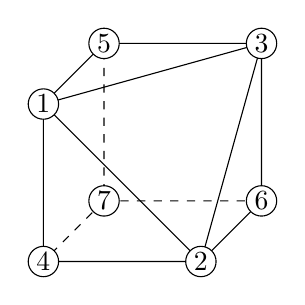
\begin{tikzpicture}[scale=2.0, line join = round]
	\coordinate (4) at (0,0,1);
	\coordinate (6) at (1,0,0);
	\coordinate (7) at (0,0,0);
	\coordinate (2) at (1,0,1);
	\coordinate (1) at (0,1,1);
	\coordinate (3) at (1,1,0);
	\coordinate (5) at (0,1,0);
	\draw (6) -- (3) -- (2) -- (1) -- (4) (5) -- (3) -- (1) -- (5) (6) -- (2) -- (4);
	\draw[dashed, thin] (6) -- (7) -- (5) (7) -- (4);
	\foreach \i in {1,...,7} {\draw (\i) node[circle, draw, fill = white, inner sep = 1pt] {\i};}
	\end{tikzpicture}
	\caption{Трехмерный куб без одной вершины}%
	\label{fig:cube7}%
\end{figure}

Решетку граней удобно визуализировать посредством диаграммы Хассе, 
представляющей собой нарисованный на плоскости граф,
вершины которого символизируют грани многогранника.
Ребрами на диаграмме Хассе соединены те и только те пары граней $f$ и $g$,
для которых одновременно выполняются следующие условия:
\begin{compactenum}
	\item[1)] $f$ является гранью $g$ (в этом случае $g$ расположена на диаграмме выше $f$);
	\item[2)] не существует грани $h$, отличающейся от $f$ и $g$, и такой, что $f$~--- грань $h$ и $h$~--- грань $g$.
\end{compactenum}
Решетка граней пирамиды над трехмерным кубом без вершины изображена на рис.~\ref{fig:cube7Hasse}.

\begin{figure}%
	\centering
	%\includegraphics[width=\columnwidth]{filename}%
	\begin{tikzpicture}[x=4mm,y=13mm,new set=import nodes, >=stealth']
	\begin{scope}[nodes={set=import nodes}] % make all nodes part of this set
	%\node (p) at (0,4) {$p_1$};
	\node[circle, draw, inner sep = 0pt, minimum size = 12pt] (polytope) at (0,4) {};
	\node[circle, draw, inner sep = 0pt, minimum size = 12pt] (emptyset) at (0,-1) {};
	\foreach \i in {1,...,8} {
		\node[circle, draw, inner sep = 0pt, minimum size = 14pt] (f\i) at ({(\i-4.5)*2.0},3) {$f_{\i}$};
	}	
	\foreach \i in {1,...,19} {
		\node[circle, draw, inner sep = 2pt] (r\i) at ({\i - 10},2) {};
	}	
	\foreach \i in {1,...,19} {
		\node[circle, draw, inner sep = 2pt] (e\i) at ({\i - 10},1) {};
	}	
	\foreach \i in {1,...,8} {
		\node[circle, draw, inner sep = 0pt, minimum size = 14pt] (v\i) at ({(\i-4.5)*2.0},0) {$v_{\i}$};
	}	
	\end{scope}
	\draw (15, 4) node[left] {весь многогранник};
	\draw (15, 3) node[left] {гиперграни};
	\draw (15, 2) node[left] {риджи};
	\draw (15, 1) node[left] {ребра};
	\draw (15, 0) node[left] {вершины};
	\draw (15, -1) node[left] {пустое множество};
	\graph {
		(import nodes); % "import" the nodes
		polytope -- {f1, f2, f3, f4, f5, f6, f7, f8};
		emptyset -- {v1, v2, v3, v4, v5, v6, v7, v8};
		e1 -- {v1, v2}; e2 -- {v1, v3}; e3 -- {v2, v3}; e4 -- {v2, v4}; e5 -- {v1, v4};
		e6 -- {v1, v5}; e7 -- {v3, v5}; e8 -- {v3, v6}; e9 -- {v2, v6}; e10 -- {v4, v7};
		e11 -- {v5, v7}; e12 -- {v6, v7};
		\foreach \i/\j in {1/13,2/14,3/15,4/16,5/17,6/18,7/19} {e\j -- {v\i, v8};};
		%\foreach \i in {1,...,14} {r\i -- e\i;}
		r1 -- {e1, e2, e3}; r2 -- {e1, e4, e5}; r3 -- {e2, e6, e7}; r4 -- {e3, e8, e9};
		r5 -- {e4, e9, e10, e12}; r6 -- {e5, e6, e10, e11}; r7 -- {e7, e8, e11, e12};
		r8 -- {e1, e13, e14}; r9 -- {e2, e14, e15}; r10 -- {e3, e13, e15}; r11 -- {e4, e13, e16}; r12 -- {e5, e14, e16};
		r13 -- {e6, e14, e17}; r14 -- {e7, e15, e17}; r15 -- {e8, e15, e18}; r16 -- {e9, e13, e18}; r17 -- {e10, e16, e19};
		r18 -- {e11, e17, e19}; r19 -- {e12, e18, e19};
		f1 -- {r1, r2, r3, r4, r5, r6, r7};
		f2 -- {r1, r8, r9, r10}; f3 -- {r2, r8, r11, r12}; f4 -- {r3, r9, r13, r14}; f5 -- {r4, r10, r15, r16};
		f7 -- {r5, r11, r16, r17, r19}; f6 -- {r6, r12, r13, r17, r18}; f8 -- {r7, r14, r15, r18, r19};
	};
	\end{tikzpicture}
	\caption{Диаграмма Хассе решетки граней пирамиды над трехмерным кубом без вершины}%
	\label{fig:cube7Hasse}%
\end{figure}
\end{comment}

Два многогранника называются \emph{комбинаторно эквивалентными}, если их решетки граней изоморфны.
Если два многогранника комбинаторно эквивалентны, то говорят, что они являются многогранниками одного \emph{комбинаторного типа}.
Свойства и числовые характеристики многогранника, однозначно определяемые его решеткой граней, называются \emph{комбинаторными}.
%, чтобы явно отличать их от других свойств и характеристик комбинаторного характера (см. замечание~\ref{rem:combinatorial} ниже).
В частности, размерность многогранника, число его вершин и число гиперграней являются комбинаторными характеристиками, а симплициальность, простота и $k$"=смежностность "--- комбинаторными свойствами.

%\begin{remark}
%\label{rem:combinatorial}
%Результаты настоящей работы лежат в области полиэдральной комбинаторики, в рамках которой комбинаторными называются не только указанные выше свойства и характеристики, но и некоторые другие, для определения которых знания решетки граней недостаточно (например, сложность расширения (см. раздел~\ref{sec:Extension})). Далее, в рассуждениях общего характера мы будем придерживаться этой традиции, но в тех случаях, когда это важно, свойства, однозначно определяемые решеткой граней, будем называть чисто комбинаторными.
%, а свойства, зависящие от геометрии многогранника, "--- \emph{комбинаторно"=геометрическими}.
%\end{remark}

Два многогранника называются \emph{двойственными} друг к другу, если их решетки граней антиизоморфны.
В частности, если $P$ и $Q$ двойственны, то вершины $P$ соответствуют гиперграням $Q$, ребра $P$ "--- риджам $Q$ и~т.\,д.
Примером двойственных многогранников могут служить $d$-куб и $d$-мерный ортаэдр.
%Многогранник, изображенный на рис.~\ref{fig:cube7}, двойственен самому себе.
%Еще одним примером двойственного самому себе многогранника является $d$-симплекс.
Вообще, многогранник, двойственный симплициальному, является простым, 
а многогранник, двойственный простому, "--- симплициальным~\cite{Emelichev:1981}.


\begin{comment}
Пусть $d$-многогранник $P$ задан в виде $P = \conv(V)$ и $\bm{0}$ является внутренней точкой этого многогранника. (Выполнения последнего условия всегда можно добиться за счет операции смещения $\bm{x} \mapsto \bm{x} + \bm{x_0}$.)
\emph{Полярой} к $P$ называется многогранник
\[
P^* \coloneqq \Set*{\bm{x}\in \R^d \given \bm{y}^T \bm{x} \le 1, \ \forall \bm{y} \in V}.
\] 
Поляра $P^*$ является примером двойственного к $P$ многогранника~\cite{Emelichev:1981,ZieglerBook}.
\end{comment}


Пусть $P$ "--- некоторый многогранник, $V = \{v_1, \dots, v_n\}$~--- множество его вершин,
а $F = \{F_1, \dots, F_k\}$~--- множество его гиперграней.
Тогда \emph{матрица инциденций вершин"=гиперграней} $M=(m_{ij})\in \{0,1\}^{n\times k}$ 
многогранника $P$ определяется следующим образом:
\[
m_{ij} = \begin{cases}
1, & \text{если } v_i \in F_j,\\
0, & \text{иначе.}
\end{cases}
\]
Матрица $M^T$ называется \emph{матрицей инциденций гиперграней"=вершин.}

Решетка граней многогранника однозначно восстанавливается по его матрице инциденций вершин"=гиперграней. 
(Один из наиболее эффективных алгоритмов решения этой задачи описан в~\cite{KaibelP:02}.)
\begin{comment}
Так, например, диаграмма Хассе на рис.~\ref{fig:cube7Hasse} восстанавливается по матрице инциденций
\begin{equation}
\begin{pmatrix}
1 & 1 & 1 & 1 & 0 & 1 & 0 & 0 \\
1 & 1 & 1 & 0 & 1 & 0 & 1 & 0 \\
1 & 1 & 0 & 1 & 1 & 0 & 0 & 1 \\
1 & 0 & 1 & 0 & 0 & 1 & 1 & 0 \\
1 & 0 & 0 & 1 & 0 & 1 & 0 & 1 \\
1 & 0 & 0 & 0 & 1 & 0 & 1 & 1 \\
1 & 0 & 0 & 0 & 0 & 1 & 1 & 1 \\
0 & 1 & 1 & 1 & 1 & 1 & 1 & 1 \\
\end{pmatrix}
\label{eq:Minc}
\end{equation}
\end{comment}
Таким образом, все 
%чисто 
комбинаторные свойства многогранника однозначно определяются по его матрице инциденций, а любые перестановки строк и/или столбцов этой матрицы не меняют этих свойств.
Легко заметить, что матрицы инциденций вершин"=гиперграней двойственных многогранников преобразуются друг в друга операцией транспонирования и, возможно, перестановкой строк и/или столбцов.
%Например, симметрия относительно побочной (дополнительной) диагонали в матрице \eqref{eq:Minc} говорит о двойственности соответствующего многогранника самому себе.


%\subsection{Аффинное и проективное преобразования многогранников}
\subsection{Аффинное отображение}

Отображение вида $\bm{x} \mapsto A \bm{x} + \bm{b}$, 
где $\bm{x} \in \R^d$, $A \in \R^{m\times d}$, $\bm{b} \in \R^m$, называется \emph{аффинным}. 
Частным случаем аффинного преобразования является \emph{ортогональная проекция} $(x_1, x_2, \dots, x_d) \mapsto (x_1, x_2, \dots, x_m, 0, \dots, 0)$, $d > m$.
Два многогранника $P\subseteq \R^d$ и $Q\subseteq \R^m$ называются \emph{аффинно эквивалентными},
если существует взаимно"=однозначное аффинное отображение $\alpha\from P \to Q$.
Из аффинной эквивалентности многогранников следует их комбинаторная эквивалентность.

Любые два $d$-симплекса аффинно эквивалентны.
Поэтому далее вместо произвольного $d$-симплекса будет рассматриваться его канонический вариант
\[
\Delta_d = \Set*{\bm{x} \in \R^{d+1} \given \bm{1}^T \bm{x} = 1, \ \bm{x} \ge \bm{0}}
= \conv\{\bm{e_1}, \dots, \bm{e_{d+1}}\}.
\]\label{ProjOfSimplex}
Нетрудно доказать, что любой многогранник, имеющий $n$ вершин, является аффинным образом симплекса $\Delta_{n-1}$.

\begin{comment}
\emph{Проективным преобразованием} называется дробно"=линейное отображение вида
\[
\tau(\bm{x}) = \frac{\alpha(\bm{x})}{\bm{a}^T \bm{x} + b},
\]
где $\alpha$ "--- аффинное отображение, размерности векторов $\bm{a}$ и $\bm{x}$ одинаковы, $b\in \R$.

Проективные преобразования обладают следующими свойствами~\cite{ZieglerBook}:
\begin{enumerate}
\item Пусть $P$ и $Q$ "--- многогранники. Если проективное преобразование $\tau \from P \to Q$ взаимно"=однозначно,	то многогранники $P$ и $Q$ комбинаторно эквивалентны.
\item Пусть многогранник $Q$ является аффинным образом некоторой грани многогранника $P$. Тогда существует проективное преобразование $\tau \from P \to Q$.
\end{enumerate}
\end{comment}
 


\section{Сложность задач и алгоритмов}
\label{sec:complexity}

Предполагается, что читатель знаком с основами теории сложности вычислений~\cite{Arora:2009, Goldreich:2008} и, в~частности, теории NP"=полных задач~\cite{Garey:1982}.
Тем не менее, чтобы избежать двусмысленности в дальнейшем, перечислим некоторые ключевые понятия и соглашения.

Для асимптотических сравнений пары функций $f\from \N \to \R_+$ и $g\from \N \to \R_+$ используются стандартные обозначения:

$f = O(g)$, если найдутся $c > 0$ и $n_0 \in \N$ такие, что $f(n) \le c \cdot g(n)$ $\forall n \ge n_0$.

$f = \Omega(g)$, если найдутся $c > 0$ и $n_0 \in \N$, что $f(n) \ge c \cdot g(n)$ $\forall n \ge n_0$.

$f = \Theta(g)$, если $f = O(g)$ и $f = \Omega(g)$.

$f = o(g)$, если $\forall c > 0$ найдется $n_c \in \N$, что $f(n) < c \cdot g(n)$ $\forall n \ge n_c$.

Функцию~$f\from \N \to \R_+$ будем называть \emph{полиномиальной} и обозначать $f(n) = \poly(n)$,
если найдется $k \in \N$, что $f(n) = O(n^k)$.
%полином $p=p(n)$ такой, что $f(n) \le p(n)$ при всех $n \in \N$.
Функция $f$ называется \emph{сверхполиномиальной},
если $f(n) = \Omega(n^k)$ для любого $k \in \N$. 
%полинома~$p$.
Так, например, функция $f(n) = a^{\ln n}$, где $a > 0$, является полиномиальной, а~функция $g(n) = a^{\ln^{1+\varepsilon} n}$ при $a > 1$ и $\varepsilon > 0$ "--- сверхполиномиальной.
Значительная часть современной теории сложности опирается на фундаментальное различие между полиномиальными и сверхполиномиальными функциями.
Точнее, речь, как правило, идет об отличии между полиномиальными функциями и~функциями вида $f(n) = \Omega\left(a^{n^{\varepsilon}}\right)$,
 где $a > 1$, $\varepsilon > 0$.
Функция $f$ называется \emph{экспоненциальной},
если $f(n) = 2^{\Theta(n)}$.
%если $f(n) = \Omega(a^n)$ при некотором $a > 1$ и, вместе с этим, $f(n) = O(2^{\poly(n)})$.
%Последние иногда называются \emph{экспоненциальными}~\cite{BondBook:2008}.

Входные данные вычислительной задачи обычно представляют
собой специальным образом упорядоченный набор чисел и меток (последние всегда можно заменить натуральными числами).
%Мы традиционно предполагаем, что входные данные вычислительной задачи кодируются в двоичную последовательность некоторым естественным образом. 
Мы традиционно предполагаем, что входные данные кодируются в двоичную последовательность $s \in \{0,1\}^* = \bigcup_{m \in \N} \{0,1\}^m$ некоторым разумным образом~\cite[с.~34--38]{Garey:1982}, \cite[p.~2]{Arora:2009}. 
%То есть вход задачи принадлежит множеству .
В частности, запись натурального числа $n$ занимает $\lceil\log_2 (n+1)\rceil$ бит.
Обозначаем: $\size(n) = \lceil\log_2 (n+1)\rceil$.
%(Традиционно, длина входа $I$ обозначается так: $|I|$. В случае, если входом является обычное (целое или рациональное) число, это создает путаницу. Поэтому в настоящей работе используется более информативное $\size(I)$.)
\begin{comment}
Соответственно, $\size(k) = \size(|k|) + 1$ для целого числа~$k$.
Рациональное число $p$ представляется парой взаимно простых чисел $k$ (числитель) и $n$ (знаменатель), где $k \in \Z$, $n \in \N$.
%, то есть $\size(p) = \size(k) + \size(n) + 1$.  
В теоретических исследованиях длина входных данных задачи обычно полагается равной сумме длин соответствующих чисел.
На практике же, чаще всего, длина входных данных пропорциональна произведению количества чисел на длину записи наибольшего из них.
Тем не менее, длина каждой из этих кодировок полиномиальна (в данном случае, не более, чем квадратична) относительно длины другой.
\end{comment}

\emph{Временн\'{о}й сложностью алгоритма} называется функция, 
которая каждому натуральному $n$ ставит в соответствие максимальное время (число операций), затрачиваемое алгоритмом для обработки входных данных длины $n$~\cite[с.~18]{Garey:1982},~\cite[p.~32]{Goldreich:2008}.
Всюду далее под \emph{сложностью алгоритма} будем понимать 
его временн\'{у}ю сложность.
Под (временн\'{о}й) \emph{сложностью задачи} будем понимать сложность (асимптотически) наиболее быстро решающего эту задачу алгоритма.
(В настоящей работе рассматриваются только разрешимые задачи.)
Сложность алгоритмов и, соответственно, задач существенно зависит от модели вычислений. Сложность задач, кроме того, может зависеть от дополнительных ограничений (мотивированных теми или иными обстоятельствами), накладываемых на класс рассматриваемых алгоритмов.

С одной стороны, согласно тезису Кобхэма--Эдмондса~\cite[c.~33]{Goldreich:2008}
(часто называемому тезисом Чёрча--Тьюринга в сильной форме~\cite[c.~26]{Arora:2009}),
любая физически реализуемая вычислительная модель 
может быть просимулирована (одноленточной) машиной Тьюринга
с (не более чем) полиномиальным увеличением времени работы.

С другой стороны, многие важные вопросы (например, соотношение классов P и NP) оказываются чрезвычайно трудными, если решать их в рамках вычислительной модели <<машина Тьюринга>>.
%~\cite[c.~259]{Arora:2009}. 
Поэтому имеет смысл обратить внимание и на другие, более удобные для изучения модели. (Кроме того, многие <<физически нереализуемые>> вычислительные модели возникают естественным образом и заслуживают изучения вне контекста упомянутых выше вопросов.) Так, например, в вычислительной модели <<дерево решений>> сложность задачи измеряется высотой дерева и всегда ограничена сверху длиной входа~\cite[c.~260]{Arora:2009}. Аналогичным образом обстоят дела и для вычислительной модели <<линейные разделяющие алгоритмы>> (см. раздел~\ref{sec:DirectTheory}). В рамках этой модели сложность любой линейной задачи комбинаторной оптимизации ограничена сверху полиномом от длины входа~\cite{Moshkov:1982}. Рассматриваемые в настоящей работе характеристики сложности задач в основном будут связаны с вычислительными моделями, имеющими геометрическую интерпретацию. Более подробному обсуждению особенностей этих моделей посвящена глава~\ref{chap:Polytopes}.

\begin{comment}
С другой стороны, все используемые в настоящее время вычислительные устройства эквивалентны в смысле тезиса Кобхэма--Эдмондса~\cite[c.~33]{Goldreich:2008},
который часто называют тезисом Чёрча--Тьюринга в сильной форме~\cite[c.~26]{Arora:2009}.

\textbf{Тезис Кобхэма--Эдмондса.}
\emph{Любая физически реализуемая вычислительная модель 
может быть просимулирована (одноленточной) машиной Тьюринга
с (не более чем) полиномиальным увеличением времени работы.}

В частности, этот тезис утверждает, что принадлежность задачи к классу $P$ (полиномиально разрешимых задач) не зависит от выбора физически реализуемой вычислительной модели.

Справедливости ради заметим, что, теоретически, с помощью квантовых вычислений можно решать задачи, принадлежность которых к классу $P$ в настоящее время не доказана.
Тем не менее, возможность физической реализации квантовых компьютеров (точнее, возможность их масштабирования) пока остается под вопросом (перспективы этого направления хорошо описаны в~\cite{Aaronson:2008}).
\end{comment}

Вычислительную задачу часто удобно представлять в виде функции, аргументами которой являются входные данные, а значением~--- решение задачи.
Функцию будем называть \emph{полиномиально вычислимой}, если соответствующая задача имеет полиномиальную сложность на машине Тьюринга.
%Функция (задача), не являющаяся полиномиально вычислимой, называется \emph{труднорешаемой}~\cite[с.~21]{Garey:1982}.

\emph{Предикатом} называется функция с множеством значений $\{\text{ложь},\text{истина}\}$ (или $\{0,1\}$).
Любой предикат $g$, заданный на множестве $\{0,1\}^*$, определяет некоторый язык
$L = \Set{x \in \{0,1\}^* \given g(x)}$, и, наоборот, любой язык $L \subseteq \{0,1\}^*$ очевидным образом определяет некоторый предикат, соответствующий задаче проверки условия $x \in L$.
Таким образом, все понятия и факты, сформулированные для языков, автоматически верны и для соответствующих предикатов.
В частности, пишем $L \in P$ ($g \in P$), если задача проверки условия $x \in L$ (вычисления предиката $g$) полиномиально вычислима.

\begin{definition}[классы NP и co-NP~{\cite{Arora:2009}}]
	\label{def:NP}
	Язык $L \subseteq\{0,1\}^*$ принадлежит классу NP, если найдется полином $p\from\N\to\N$ и полиномиально вычислимый предикат $g\from \{0,1\}^* \times \{0,1\}^* \to \{\text{ложь},\text{истина}\}$
	такие, что для каждого $x \in \{0,1\}^*$
	\[
	x\in L \iff \text{найдется } u\in \{0,1\}^{p(\size(x))} 
	\text{ такой, что } g(x,u).
	\]

Язык $L$ принадлежит классу co-NP, если язык $\{0,1\}^* \setminus L$ принадлежит NP.

Говорят, что задача проверки условия $x \in L$ принадлежит классу NP (co"~NP),
если язык $L$ принадлежит этому классу.
\end{definition}

Классическое понятие полиномиальной сводимости может определяться по разному в зависимости от типа решаемых задач~\cite{Garey:1982, Goldreich:2008}.
Чтобы избежать излишних (с точки зрения основных результатов диссертации) подробностей, везде далее, если не оговорено иное, под полиномиальной сводимостью мы будем понимать полиномиальную сводимость по Тьюрингу (иногда она называется сводимостью по Куку).
Приведем наиболее короткое определение этого типа сводимости, предполагающее, что читатель знаком с понятием оракульной машины Тьюринга~\cite{Garey:1982, Goldreich:2008}:

\begin{definition}[полиномиальная сводимость]
	Задача $\Pi$ \emph{полиномиально сводится} к задаче $\Pi'$,
	если существует оракульная машина $M$ такая, что для любой функции $f$, решающей задачу $\Pi'$, машина $M$ с оракулом $f$ решает задачу $\Pi$ за полиномиальное время. (Обращение к оракулу $f$ выполняется за единицу времени.)
\end{definition}

Задача из класса NP (co-NP) называется \emph{NP-полной} (\emph{co-NP-полной}),
если любая другая задача из этого класса полиномиально сводится к ней.

%Мы не приводим здесь определения классов NP и co-NP, а также понятия NP-полной (и co-NP-полной) задачи~\cite{Garey:1982}, так как эти термины являются устоявшимся и понимаются всеми специалистами одинаково (в отличие, например, от понятия NP-трудной задачи).

В качестве примера приведем формулировку наиболее известной NP-полной задачи о выполнимости булевой формулы~\cite[с.~56]{Garey:1982}.

Пусть $U = \{u_1, u_2, \ldots, u_k\}$ "---
множество булевых переменных. 
Каждая булева переменная может принимать лишь одно из двух значений: 
$1$ или $0$.
%$1 \overset{\text{def}}{=} \text{<<истина>>}$ или $0 \overset{\text{def}}{=} \text{<<ложь>>}$.
Если $u\in U$, то $u$ и $\bar{u}$, $\bar{u} = 1 - u$, называются \emph{литералами}.
Множество литералов, например $\{u_2, \bar{u}_4, u_5\}$,
называется \emph{дизъюнкцией} над $U$ и обычно обозначается $u_2 \vee \bar{u}_4 \vee u_5$.
Говорят, что дизъюнкция \emph{выполнена} (принимает значение 1) при некотором наборе значений переменных, если хотя бы один из входящих в нее литералов
равен 1.
Пусть $C = \{D_1, D_2, \ldots, D_m\}$ "--- некоторый набор дизъюнкций, далее называемый \emph{конъюнкцией}.
В таких случаях говорят, что булева формула $C$ задана в \emph{конъюнктивной нормальной форме}\label{def:CNF} (КНФ).
Конъюнкция $C$ называется \emph{выполнимой}, если существует набор значений переменных такой, что выполненными оказываются все дизъюнкции из $C$.
\medskip

\problem{Задача о выполнимости.}
Дано множество переменных $U$ и конъюнкция~$C$ над $U$.
Верно ли, что $C$ выполнима?
\medskip

%В рамках теории NP-задач задачей называется множество всех входных данных (в данном случае конъюнкций) для которых ответ на вопрос задачи положителен.
%Это множество обычно называется языком, а входные данные отдельно взятой индивидуальной задачи "--- словом~\cite{Garey:1982}.
Исторически задача о выполнимости оказалась первой NP-полной задачей (хотя сам термин возник позднее)~\cite{Cook:1971}.
\emph{Задача о $k$-выполнимости} представляет собой частный случай задачи о выполнимости, когда каждая дизъюнкция содержит ровно $k$ литералов.
Так как для любого натурального $k \ge 3$ задача о выполнимости полиномиально сводится~\cite{Karp:1972} к задаче о $k$-выполнимости, то последняя также является NP-полной.

\emph{NP-трудными} задачами будем называть те, к которым полиномиально сводятся NP-полные задачи.
Заметим, что некоторые исследователи при определении NP-трудной задачи предпочитают использовать сводимость по Карпу. 
В этом случае, в частности, классы NP-трудных и co-NP-трудных задач отличаются друг от друга при условии $\NP \ne \coNP$.
Мы же далее будем предполагать использование полиномиальной сводимости по Тьюрингу. 
При таком определении co-NP-полные задачи являются NP-трудными.

\begin{comment}
Далее нам также потребуется определение класса $D^p$~\cite{PapadimitriouY:1984}:
\[
D^p = \{L_1 \cap L_2 \mid L_1\in \NP, \ L_2\in \coNP\}.
\]
В частности, NP и co-NP являются подмножествами $D^p$, откуда следует, что все $D^p$-полные задачи являются NP-трудными.
В качестве примера приведем две $D^p$-полные задачи~\cite{PapadimitriouY:1984}:
\begin{enumerate}
	\item \problem{Выполнимость--невыполнимость.} Даны две булевы формулы. Верно ли, что первая выполнима, а вторая "--- невыполнима.
	\item \problem{Точная клика.} Дан граф $G$ и число $k \in \N$. Верно ли, что $k$ является кликовым числом этого графа.
\end{enumerate}
\end{comment}



\section{Задачи комбинаторной оптимизации}
\label{sec:CO}

В трехтомнике A. Schrijver ``Combinatorial optimization'' (2003) приводится следующее определение комбинаторной оптимизации: <<Комбинаторная оптимизация ищет оптимальный объект в конечном множестве объектов>>~\cite[p.~1]{SchrijverCO:2003}. Попытки дать более точное определение, учитывающее особенности прикладных задач и, вместе с тем, позволяющее делать теоретические выводы о свойствах массовых задач, приводят к определению класса NPO (NP optimization)~\cite{Ausiello:2011, Momke:2009}.

%http://www.nada.kth.se/~viggo/problemlist/
\begin{definition} %[задача комбинаторной оптимизации]
\label{def:COP}
\emph{Задача из класса NPO} представляет собой четверку:
\begin{enumerate}
	\item \emph{Язык входных данных} $L$, $L \in P$. Каждое слово $I \in L$ называется \emph{входными данными} задачи.
	\item \emph{Предикат допустимости} $g = g(x, I) \in \{\text{ложь}, \text{истина}\}$, определяющий \emph{множество допустимых решений} 
	\[X = X(I) = \Set*{x \in \{0,1\}^* \given \size(x) = \poly(\size(I)) \text{ и } g(x, I)}.\]
	\item \emph{Целевая функция} $f = f(x, I) \in \Q$, где $x \in X$.
	\item \emph{Направление оптимизации:} $\min$ или $\max$.  По умолчанию, $\max$.
\end{enumerate}
Предикат $g$ и целевая функция $f$ полиномиально вычислимы.
Если входные данные $I$ не зафиксированы, то задача называется \emph{массовой}, иначе "--- \emph{индивидуальной} (или \emph{экземпляром} задачи).
Цель задачи "--- среди всех допустимых решений $X$ найти такое, на котором целевая функция $f$ принимает оптимальное значение ($\min$ или $\max$ в соответствии с направлением оптимизации).
\end{definition}

Основным объектом исследований настоящей работы являются задачи комбинаторной оптимизации с линейной целевой функцией. 
%В [\cite{Junger:1995,Onn:2004}] линейной задачей комбинаторной оптимизации называется задача оптимизации на подмножествах множества E

\begin{definition}
\label{def:LCOP}
\emph{Линейная задача комбинаторной оптимизации} представляет собой четверку:
\begin{enumerate}
	\item Язык входных данных $L$, $L \in P$. Далее слово $I \in L$ называется \emph{кодом задачи}.
	\item \emph{Размерность} $d \from L \to \N$.
	\item Предикат допустимости $g \from \Z^d \times L \to \{\text{ложь}, \text{истина}\}$, определяющий множество допустимых решений 
	\[X = X(I) = \Set*{\bm{x} \in \Z^d \given \size(\bm{x}) = \poly(\size(I) + d(I)) \text{ и } g(\bm{x}, I)}.\]
	\item Направление оптимизации: $\min$ или $\max$. По умолчанию, $\max$.
\end{enumerate}
Как и прежде, предполагается, что функции $d$ и $g$ полиномиально вычислимы.
Входными данными индивидуальной задачи являются её код $I$ и \emph{целевой вектор} $\bm{c} \in \Q^d$.
Целевая функция линейна: $f(\bm{x}, \bm{c}) = \bm{c}^T \bm{x}$, где $\bm{x} \in X$.
\end{definition}

\begin{comment}
\begin{remark}
	\label{rem:CombOpt4}
	%Функции $d = d(I)$, $S = S(I)$ и $g = g(u,I)$ определяют множество допустимых решений соответствующей задачи. Предикат входных данных может быть встроен в эти функции таким образом, чтобы для недопустимого входа множество решений было бы пустым. 
	%По этой причине 
	В дальнейшем, при описании задач мы не рассматриваем язык входных данных, предполагая, что на вход задачи подаются только допустимые данные.
	Учитывая, что направление оптимизации по умолчанию "--- максимум, линейная задача комбинаторной оптимизации будет определяться не четверкой, а~парой функций: размерностью $d = d(I)$ и предикатом допустимости $g = g(x, I)$.
\end{remark}
\end{comment}

\begin{remark}
Задача минимизации всегда может быть преобразована в задачу максимизации (и наоборот) с помощью замены $\bm{c} \coloneqq -\bm{c}$.
Учитывая это обстоятельство, далее мы в основном будем рассматривать задачи на максимум, а линейной задачей комбинаторной оптимизации называть тройку $(L,d,g)$.
\end{remark}

\begin{remark}
Умножение целевого вектора $\bm{c}$ на положительный скаляр не~меняет оптимальности решений. 
Кроме того, за счет умножения $\bm{c}$ на наименьшее общее кратное знаменателей его компонент, его можно сделать целочисленным за полиномиальное относительно размера $\size(\bm{c})$ время.
Поэтому, не уменьшая общности, можно предполагать, что вектор $\bm{c}$ "--- целочисленный.
\end{remark}


В качестве примера рассмотрим классическую задачу о рюкзаке. 
Даны $n$ предметов и для каждого из них известны размер $a_i \in \Z$ и стоимость $c_i \in \Z$. Кроме того, известен размер рюкзака $b \in \Z$.
Требуется выбрать подмножество предметов так, чтобы их суммарный размер был меньше размера рюкзака, а их суммарная стоимость была бы максимальной.

Чтобы представить эту задачу в виде линейной задачи комбинаторной оптимизации, каждому подмножеству $s \subseteq [n]$ поставим в соответствие его характеристический вектор $\bm{x} = \chi(s) \in \{0,1\}^n$. При такой интерпретации, в задаче требуется найти $\bm{x} \in \{0,1\}^n$, доставляющий максимальное значение функции $\bm{c}^T \bm{x}$, где $\bm{c} = (c_i) \in \Z^n$ "--- вектор стоимостей предметов, при условии $\bm{a}^T \bm{x} \le b$, где $\bm{a} = (a_i) \in \Z^n$ "--- вектор размеров предметов.
В обозначениях определения~\ref{def:LCOP}, код задачи состоит из тройки $(n, \bm{a}, b)$, размерность $d = n$, а предикат $g$ проверяет справедливость условий $\bm{a}^T \bm{x} \le b$ и $\bm{x} \in \{0,1\}^n$. Далее будем предполагать, что размерность $n$ вектора $\bm{a}$ содержится в его описании. Это позволяет исключить из кода задачи избыточный параметр $n$.


%,Onn:2004
Далее мы будем рассматривать \emph{только} линейные задачи комбинаторной оптимизации, называя их, для краткости, задачами комбинаторной оптимизации.
С одной стороны, задачи с таким ограничением довольно часто встречаются на практике~\cite{Junger:1995}.
%: оптимизационные задачи на графах (кратчайший путь, коммивояжер и т.п.), задача о рюкзаке, задача целочисленного линейного программирования и многие другие.
С другой стороны, методы решения задач такого типа в настоящее время развиты настолько сильно, что даже задачи с нелинейной целевой функцией во многих случаях решаются более эффективно, если привести их к линейному виду.
В качестве примера покажем, как выполняется это преобразование для некоторых, наиболее популярных задач.

\problem{Задача булева квадратичного программирования.}
Дан набор (рациональных) коэффициентов многочлена 
\[
p(\bm{x}) = \sum\limits_{\mathclap{1\le i \le j \le n}} c_{ij} x_i x_j, 
\quad \bm{x} = (x_1, \dots, x_n) \in \{0, 1\}^n. 
\]
Требуется найти $\bm{x}$, при котором $p(\bm{x})$ достигает максимума.

С целью линеаризации в этой задаче вместо вектора $\bm{x} = (x_1, \dots, x_n) \in \{0, 1\}^n$ рассматривается вектор $\bm{y} \in \{0, 1\}^{n(n+1)/2}$ с координатами $y_{ij} = x_i x_j$, $1 \le i \le j \le n$.
В этом случае размерность $d = n(n+1)/2$, предикат допустимости проверяет выполнение условий $y_{ij} = y_{ii} y_{jj}$ и $y_{ij} \in \{0,1\}$,
а целевая функция становится линейной: $f(\bm{y}) = \sum_{1\le i \le j \le n} c_{ij} y_{ij}$.

\problem{Задача поиска максимума многочлена на множестве целых точек отрезка.}
\label{def:PolyMax}
Даны: набор (рациональных) коэффициентов многочлена $p(x) = \sum_{k = 1}^d c_k x^k$
и два целых $a, b \in \Z$, $a \le b$.
Найти целое $x \in [a, b]$ при котором $p(x)$ принимает наибольшее значение.

По аналогии с предыдущей задачей, в задаче поиска максимума многочлена можно вместо переменной $x \in \Z$ рассмотреть вектор $\bm{y} \in \Z^d$, координаты которого удовлетворяют условию $y_k = y_1^k$, $k \in [d]$. Тогда целевая функция $f(\bm{y}) = \sum_{k=1}^{d} c_k y_k$.

% Очень хорошее описание линейных задач комбинаторной оптимизации и целочисленного программирования есть в \cite{Junger:1995} "Practical problem solving with cutting plane algorithms in combinatorial optimization"
% Здесь же эти задачи называются NP-трудными

Довольно часто множество линейных задач комбинаторной оптимизации дополнительно ограничивается условием $\bm{x} \in \{0,1\}^d$. Это связано с тем, что многие прикладные задачи допускают следующую формулировку~\cite{Junger:1995,Onn:2004}.
Дано конечное множество $E$, предикат допустимости $g\from 2^E \to \{\text{ложь}, \text{истина}\}$ и функция весов $c\from E \to \Q$.
Для каждого подмножества $T\subseteq E$ определено
значение целевой функции $f(T) = \sum_{e\in T} c(e)$.
Требуется найти
\(T^* = \argmax_{T\subseteq E}\Set{f(T) \given g(T)}\).
Множество допустимых решений такой задачи состоит из характеристических векторов  подмножеств множества $E$, для которых $g$ принимает значение <<истина>>.

Другим, часто встречающимся типом ограничений, являются ограничения, накладываемые на выбор целевого вектора. В терминологии определения~\ref{def:COP}, выполнение этих условий закладывается в язык входных данных.
Во многих задачах эти ограничения являются линейными.
Примером может служить классическая задача о кратчайшем пути, в которой ограничения неотрицательности длин участков дорог, то есть $\bm{c} \ge \bm{0}$, переводят задачу из класса NP-трудных в класс полиномиально разрешимых~\cite[sec.~7.5b, 8.6b]{SchrijverCO:2003}.
Далее будем называть такие задачи линейными задачами комбинаторной оптимизации \emph{с ограничением на множество исходных данных (целевых векторов)}.
В~общем случае, ниже речь пойдет о проверяемых за полиномиальное время ограничениях вида $\bm{c} \in P$, где $P=P(I)$ "--- некоторый полиэдр.
(В~случае задачи о кратчайшем пути, $P = \R^d_+$.)

